% Fault tolerant control of a redundant cable driven parallel robot
% International Journal of Control (Taylor & Francis), Interact layout with author-date references.
% Compile with pdflatex and BibTeX. The switch below gives the anonymous version for double
% anonymous review (\blindtrue) or the version with the author details (\blindfalse).
\documentclass{interact}

\newif\ifblind
\blindtrue
\ifdefined\fullversion\blindfalse\fi

\usepackage{amssymb}
\usepackage{bm}
\usepackage{array}
\usepackage{graphicx}
\usepackage{algorithm}
\usepackage[noend]{algpseudocode}
\usepackage{url}
\usepackage{natbib}
\bibpunct[, ]{(}{)}{;}{a}{}{,}
\renewcommand\bibfont{\fontsize{10}{12}\selectfont}

\graphicspath{{figures/}}
\newcommand{\vc}[1]{\bm{#1}}
\newcommand{\mt}[1]{\mathbf{#1}}
\newcommand{\sk}[1]{[#1]_{\times}}
\newcommand{\eye}{\mt{I}}
\renewcommand{\algorithmicrequire}{\textbf{Every 1 ms:}}

\begin{document}

\articletype{Original article}

\title{Fault tolerant control of a redundant cable driven parallel robot with model based fault isolation and precomputed recovery plans}

\ifblind
\maketitle
\else
\author{
\name{Mfeuter Joseph Tachia\textsuperscript{a}\thanks{CONTACT M.\,J. Tachia. Email: m.tachia@innopolis.university. ORCID: M.\,J. Tachia 0000-0002-9274-3658; A.\,V. Maloletov 0000-0002-7312-2944} and Alexander V. Maloletov\textsuperscript{a,b}}
\affil{\textsuperscript{a}Research Center of the Artificial Intelligence Institute, Innopolis University, Innopolis, Russia; \textsuperscript{b}Volgograd State Technical University, Lenin Avenue~28, Volgograd, Russia}
}
\maketitle
\fi

\begin{abstract}
A cable driven parallel robot that loses a cable has a fraction of a second to move its platform to a pose the remaining cables can hold. We present a fault tolerant controller for the eight cable robot IPAnema~2. Extended state observers at the winches and an interacting multiple model estimator over seventeen modes isolate cable breaks and actuator faults from the motor encoders and currents alone, and a model predictive controller answers a declared break with a recovery plan computed in advance. In 624 simulated fault runs, the controller declared every break within 19~ms and lost the platform after 11 of 208 breaks, against 122 without fault tolerance. Weighting the fault scenarios by their probabilities did not help. The results assume that each solution of the predictive controller acts within its 20~ms period; delayed by one period, the platform fell in every run tested.
\end{abstract}

\begin{keywords}
Cable driven parallel robot; fault tolerant control; fault isolation; interacting multiple model; model predictive control; recovery planning
\end{keywords}

\noindent{\small Word count: about 9,850 words in Sections 1 to 8 (about 10,450 with the tables, figure captions and algorithm), without the abstract, equations, references and appendix.}

\section{Introduction}\label{sec:intro}

A cable driven parallel robot can lose a cable in the middle of a task, and when it does, the platform starts to fall before any controller has noticed. These robots move a platform with cables wound on winches fixed to a frame, which gives them a workspace of several metres, a light moving mass and a payload that rigid parallel robots of the same size cannot reach \citep{pott2018book,zarebidoki2022review,tachia2026review}. These properties are the reason they are considered for building facades, large scale additive manufacturing and other construction tasks \citep{izard2017printing}, and they are also the reason a failure is dangerous: a platform of several kilograms hangs metres above the floor, held by thin cables and by drives that run for hours. A cable can break, and a winch can lose part of its torque or develop a parasitic one. In a fully constrained robot with eight cables and six degrees of freedom the loss of one cable does not make the platform uncontrollable at once, but it removes most of the poses at which the remaining cables can hold it. For the robot of this study, IPAnema~2 \citep{pott2013ipanema}, no level pose near the task can be held after an upper cable breaks (Section~\ref{sec:workspace}), and without a fault tolerant reaction the platform was lost after every one of 104 simulated breaks of an upper cable. Recovering from a break is therefore a race. The controller has to find out which cable has gone, decide where the platform can still be held and start moving it there within a few tenths of a second, while the platform is already falling.

Most work on cable failures asks what the robot can still do once the failure is known. For the motion after a break, \citet{berti2016recovery} moved the point mass of a redundant suspended robot from the unstable pose left by the failure to a new static equilibrium, \citet{passarini2019camera} drove a cable suspended camera toward a safe landing pose along an oscillatory trajectory that keeps the remaining tensions positive and bounded, and \citet{boschetti2019rehab} stopped a rehabilitation robot with a wrench opposed to its motion; \citet{boschetti2021experimental} later tested a recovery strategy on a suspended robot with three degrees of freedom. \citet{boumann2019emergency} developed emergency strategies that minimise the kinetic energy of the platform or steer it with potential fields, and validated them later on a prototype \citep{boumann2023validation}, while \citet{dipaola2024smapid} guided the load inside the remaining wrench feasible workspace with a sliding mode adaptive PID control. These strategies take the failure as known at its onset, and most of them were shown on planar or point mass models or on suspended robots. For a spatial, fully constrained robot two questions are left open: how the delay and the reliability of the diagnosis shape the outcome, and how a recovery motion of the full six degree of freedom pose, which has to be dynamically feasible with seven cables, can be ready within the few tenths of a second the platform leaves.

Banks of mode matched filters combined by the interacting multiple model (IMM) estimator \citep{blom1988imm} have long been used to detect and isolate actuator and sensor failures \citep{zhang1998imm}. In cable driven robots the diagnosis has received less attention than the recovery. \citet{raman2023cable} isolated cable failures of a planar reconfigurable robot with an IMM bank of extended Kalman filters, assuming that the platform pose is measured. \citet{majdi2023smc} detected partial actuator losses of a planar robot with an extended state observer, \citet{marufkhani2023sdre} detected and estimated faults of a planar robot with a state dependent Riccati equation approach, and \citet{fazeli2023active} estimated actuator faults with an adaptive observer inside a finite time sliding mode controller and verified the scheme on a planar robot. \citet{bettega2025load} estimated the load torque of each motor from its current and encoder and detected cable failures with machine learning classifiers. Learned detectors need no model of the faulty robot, but they know only the behaviour represented in their training data \citep{khalastchi2019survey}, and in a fault tolerant controller that behaviour changes as soon as the controller acts on the detector. None of these works isolates both cable breaks and actuator faults of a spatial robot from the winch signals alone, and we have not found a comparison of a learned and a model based diagnosis inside the same closed loop.

Model predictive control (MPC) suits cable robots because the tension bounds become constraints of the optimisation instead of being left to a separate tension distribution step \citep{gouttefarde2015tda}. \citet{santos2022nmpc} built the tension distribution into a nonlinear MPC with conditions for stability, \citet{song2022wmpc} used an offline workspace analysis to give the online problem convex constraints and recursive feasibility, \citet{bettega2023mpc} computed bounded tensions for path tracking with flexible cables by an MPC, and \citet{gao2025dobmpc} combined MPC with a disturbance observer. When the model itself is uncertain, multistage MPC optimises one input sequence against several candidate models at once \citep{lucia2013multistage}. A diagnosis that returns mode probabilities suggests combining the two: before a fault is confirmed, the controller could already weigh what each plausible fault would do and move the platform toward poses that would survive it. This was the hypothesis our study began with, and here it is tested as an ablation.

This paper presents and evaluates a fault tolerant controller for IPAnema~2 on a simulator that integrates elastic and unilateral cables, the winch dynamics, sensor quantisation and noise and randomised parameters, while the controller works with a rigid cable model. An extended state observer at each winch estimates the cable tension from the encoder and the motor current, and an IMM over seventeen modes, the healthy robot, eight cable breaks and eight actuator faults, separates breaks from actuator faults at the platform. An MPC tracks the task within the tension bounds, and after a break is declared it follows a recovery plan, the solution of an optimal control problem on the seven cable model computed in advance along the known task. All methods ran on the same randomised runs, with the endpoints, the statistics and the settings of every method fixed before the evaluation and one documented amendment of the threshold baseline (Section~\ref{sec:simulator}). The contributions are three.
\begin{enumerate}
\item A two level diagnosis that isolates cable breaks, losses of effectiveness and torque biases of a spatial robot from the encoders and motor currents of the winches, without load cells or a pose sensor. It identified 623 of 624 faults correctly and declared every break within 19~ms.
\item A library of recovery plans computed offline along the task and selected at the declaration, which removes the latency of solving the plan online. With it the platform was lost after 11 of 208 breaks, against 20 with the same planner solved online and 122 without fault tolerance.
\item Paired evidence on when weighting the fault scenarios of the MPC by their probabilities before a declaration can act. With the IMM it changed no safety endpoint, because every break was declared within one period of the MPC. With a recurrent classifier that shares the state estimator of the IMM and was trained on the same signals, the weighting came with false alarms in 154 of 252 runs and with unsuccessful solves of the MPC, and the platform was lost in 44 of 64 break runs.
\end{enumerate}
We do not claim new theory for the observers, the estimator or the MPC; the contribution is their combination for a spatial robot that has neither load cells nor a pose sensor, and the paired evidence on what it achieves. All results are simulations in which each computation is available at its sample, and Section~\ref{sec:latency} shows that the controller depends on this: with the output of the MPC one period late, the platform fell before any fault.

% =====================================================================
\section{Robot, model and faults}\label{sec:model}

\subsection{The robot}\label{sec:robot}

IPAnema~2 is a member of a family of industrial cable robots, built in a frame of $8\times6\times5$~m \citep{pott2013ipanema}. We use its geometry, mass, inertia and upper tension bound as distributed with the IPAnema~2 model of the open source toolkit CASPR \citep{lau2016caspr}, whose geometry coincides with the published one, and its cables, winches and drives as published (Table~\ref{tab:parameters}). Anchor $i$ is at $\vc a_i=(4\sigma_{x,i},\,3\sigma_{y,i},\,z_{a})$~m, with $z_a=5$~m for the upper cables 1 to 4 and $z_a=1$~m for the lower cables 5 to 8, and the cable is attached to the platform at $\vc b_i=(0.65\sigma_{x,i},\,0.125\sigma_{y,i},\,0.25)$~m for the upper and $(0.75\sigma_{x,i},\,0.10\sigma_{y,i},\,0.75)$~m for the lower cables, where the signs $(\sigma_{x,i},\sigma_{y,i})$ are $(-,+)$, $(+,+)$, $(+,-)$ and $(-,-)$ for cables 1 to 4 and, in the same order, for cables 5 to 8. The platform of 10~kg has its centre of mass 0.5~m above its reference point $P$, the point that follows the task, and the home pose places $P$ at $(0,0,3)$~m with zero orientation (Fig.~\ref{fig:robot}). With eight cables pulling upward and downward at the same time the platform resists a wrench in any direction while every cable stays in tension. The redundancy is two, which leaves a two dimensional family of tension distributions for every wrench, and after the loss of one cable it drops to one.

% written by scripts/paper_tables.py from stored files; do not edit
\begin{table}
\tbl{Model of the robot. The controller uses the nominal values; the plant of every run draws the randomised ones from the seed of the run.}
{\begin{tabular}{@{}p{0.2\linewidth}p{0.47\linewidth}p{0.27\linewidth}@{}}
\toprule
Quantity & Value & Source \\
\midrule
Frame (anchor box) & $8\times6$ m, anchors at $z=1$ and $5$ m & CASPR model IPAnema\_2 \cite{lau2016caspr} \\
Platform attachments & $|x|\le0.75$, $|y|\le0.125$, $z\in[0.25,0.75]$ m & CASPR \\
Mass, inertia & 10 kg, 1 kg\,m$^2$ per axis & CASPR \\
Tension bounds & $t_{\min}=10$ N, $t_{\max}=200$ N & CASPR ($t_{\max}$); design choice ($t_{\min}$) \\
Cable & Dyneema, $d=1.5$ mm, $EA=35188$ N, retardation 20 ms & \cite{pott2013ipanema}; EA scaled from \cite{tempel2015iftomm} \\
Drum, gearbox & radius 50 mm, $i=12$, stroke 6 m & \cite{pott2013ipanema} \\
Motor & MSK030C: 0.9 N\,m rated, 4 N\,m peak, rotor $3\times10^{-5}$ kg\,m$^2$ & sized from \cite{rexroth_msk2018} \\
Velocity, acceleration limits & 2.5 m/s, 25 m/s$^2$ & \cite{pott2013ipanema} \\
Encoder & 1048576 counts/rev, $\pm$120 arcsec & \cite{rexroth_msk2018}, option M1 \\
Motor current noise & 0.004 N\,m (nominal), $\times2$ in half of the runs & design choice \\
Rates & plant RK4 step 62.5 $\mu$s, control 1000 Hz, measurement delay 1 sample & step convergence study \\
Randomised in every run & mass $\pm10\%$, principal inertias $\pm20\%$, centre of mass $\pm2$ cm, anchors $\pm5$ mm, $EA\ \pm20\%$ (uniform) & study design \\
\bottomrule
\end{tabular}}
\label{tab:parameters}
\end{table}


\begin{figure}
\centering
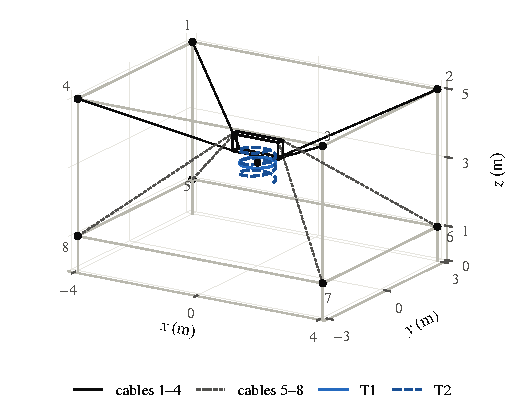
\includegraphics{fig01_robot_task}
\caption{IPAnema~2 at its home pose, with the eight cables (upper anchors at $z=5$~m, lower anchors at $z=1$~m), the reference point P of the platform and the two reference paths: the circle T1 and the helix T2, both 16~s long.}\label{fig:robot}
\end{figure}

\subsection{Kinematics}\label{sec:kinematics}

The world frame has its $z$ axis pointing upward. The pose of the platform is described by the generalised coordinates
\begin{equation}\label{eq:q}
\vc q=\begin{bmatrix}\vc p\\ \vc\varphi\end{bmatrix}\in\mathbb R^{6},\qquad \mt R(\vc\varphi)=\mt R_z(\psi)\,\mt R_y(\vartheta)\,\mt R_x(\phi),
\end{equation}
where $\vc p$ is the position of $P$ and $\vc\varphi=[\phi,\vartheta,\psi]^\top$ are ZYX Euler angles. Each cable is taken to leave the frame at its fixed anchor point, and the small motion of the exit point on the guiding pulley is neglected. The angular velocity follows from the Euler rates as $\vc\omega=\mt E(\vc\varphi)\dot{\vc\varphi}$, with $\mt E$ singular only at $\vartheta=\pm\pi/2$, far outside the tilt this robot can hold, and we collect the velocities in the twist $\vc\nu=[\dot{\vc p}^\top,\vc\omega^\top]^\top=\mt H(\vc q)\dot{\vc q}$ with $\mt H=\operatorname{blkdiag}(\eye_3,\mt E)$. Cable $i$ runs from the attachment point to the anchor, so its vector, length and direction are
\begin{equation}\label{eq:cable}
\vc l_i=\vc a_i-\vc p-\mt R\vc b_i,\qquad l_i=\lVert\vc l_i\rVert,\qquad \vc u_i=\vc l_i/l_i,
\end{equation}
and a tension $t_i\ge0$ acts on the platform as the force $t_i\vc u_i$. Differentiating \eqref{eq:cable} gives, for all cables together,
\begin{equation}\label{eq:ldot}
\dot{\vc l}=-\mt W^\top\vc\nu,\qquad
\mt W=\begin{bmatrix}\vc u_1&\cdots&\vc u_n\\ (\mt R\vc b_1)\times\vc u_1&\cdots&(\mt R\vc b_n)\times\vc u_n\end{bmatrix},
\end{equation}
where $\mt W\in\mathbb R^{6\times n}$ is the wrench matrix: the cables apply to the platform the force and the moment about $P$ given by $\mt W\vc t$. The same matrix, transposed and with a minus sign, maps the twist to the rates of the cable lengths, and the sign in \eqref{eq:ldot} is the one that keeps the cables pulling.

\subsection{Dynamics from the Lagrange equations}\label{sec:lagrange}

We treat the platform as a rigid body and the cables, in this subsection, as sources of generalised forces. With $\vc c_w=\mt R\vc c$ the position of the centre of mass relative to $P$, the kinetic and potential energies are
\begin{align}
T&=\tfrac12 m\lVert\dot{\vc p}+\vc\omega\times\vc c_w\rVert^2+\tfrac12\vc\omega^\top\mt I_c\vc\omega=\tfrac12\dot{\vc q}^\top\mt M(\vc q)\dot{\vc q},\label{eq:T}\\
V&=m g\,\vc e_3^\top(\vc p+\mt R\vc c),\label{eq:V}
\end{align}
where $\mt I_c=\mt R\mt I_G\mt R^\top$ is the inertia about the centre of mass in world coordinates, and expanding the square gives
\begin{equation}\label{eq:M}
\mt M=\mt H^\top\mt M_\nu\mt H,\qquad
\mt M_\nu=\begin{bmatrix}m\eye_3&-m\sk{\vc c_w}\\ m\sk{\vc c_w}&\mt I_c-m\sk{\vc c_w}^2\end{bmatrix},
\end{equation}
with $\sk{\cdot}$ the cross product matrix. The off diagonal blocks couple translation and rotation because $P$ is not the centre of mass, and with an offset of 0.5~m this coupling is far from small. The elastic energy of the cables is deliberately left out of $V$: the cable forces enter once, through their virtual work, so that they cannot be counted both as a potential and as an applied force. A virtual displacement moves attachment point $i$ by $\delta\vc p+\delta\vc\Theta\times\mt R\vc b_i$ with $\delta\vc\Theta=\mt E\,\delta\vc\varphi$, and the virtual work of the tensions,
\begin{equation}\label{eq:Q}
\delta W=\sum_{i=1}^n t_i\vc u_i^\top(\delta\vc p+\delta\vc\Theta\times\mt R\vc b_i)=(\mt H^\top\mt W\vc t)^\top\delta\vc q,
\end{equation}
gives the generalised force $\vc Q=\mt H^\top\mt W\vc t=-(\partial\vc l/\partial\vc q)^\top\vc t$, which says that a tension does negative work when its cable gets longer. The Lagrange equations of $L=T-V$ then read
\begin{equation}\label{eq:EL}
\mt M(\vc q)\ddot{\vc q}+\mt C(\vc q,\dot{\vc q})\dot{\vc q}+\vc G(\vc q)=\mt H^\top\mt W\vc t,
\end{equation}
where $\vc G=\partial V/\partial\vc q=-\mt H^\top\vc w_g$ with the gravity wrench $\vc w_g=[m\vc g^\top,\ (\vc c_w\times m\vc g)^\top]^\top$, and $\mt C$ is built from the Christoffel symbols of the first kind,
\begin{equation}\label{eq:C}
C_{kj}=\sum_{i=1}^{6}\frac12\Big(\frac{\partial M_{kj}}{\partial q_i}+\frac{\partial M_{ki}}{\partial q_j}-\frac{\partial M_{ij}}{\partial q_k}\Big)\dot q_i,
\end{equation}
the choice that makes $\dot{\mt M}-2\mt C$ skew symmetric. Substituting $\dot{\vc q}=\mt H^{-1}\vc\nu$ and multiplying by $\mt H^{-\top}$ gives the Newton--Euler form about $P$,
\begin{equation}\label{eq:NE}
\begin{gathered}
\mt M_\nu\dot{\vc\nu}+\vc b(\vc q,\vc\nu)=\mt W\vc t+\vc w_g,\\
\vc b=\begin{bmatrix}m\,\vc\omega\times(\vc\omega\times\vc c_w)\\ \vc\omega\times\mt I_c\vc\omega+m\,\vc c_w\times\big(\vc\omega\times(\vc\omega\times\vc c_w)\big)\end{bmatrix},
\end{gathered}
\end{equation}
which has no Euler angle singularity in its mass matrix and is cheaper to evaluate. The simulator integrates \eqref{eq:NE} with the orientation carried as a unit quaternion, so that it stays regular through the large rotations of an uncontrolled platform, and the estimators and the controller use the same equation with the tensions as inputs. We checked the derivation against a symbolic Lagrangian and the two forms against each other numerically (Appendix~\ref{app:verification}).

\subsection{Cables and winches}\label{sec:cables}

Each cable is wound on a drum that a motor turns through a gearbox. With the motor angle $\theta_i$ taken positive when cable is reeled in, the unstretched free length is $l_{u,i}=l^0_{u,i}-r_d\theta_i$, where $r_d=r_D/i_g=50~\text{mm}/12=4.167$~mm/rad is the cable paid out per radian of the motor shaft. With the stretch $\Delta_i=l_i-l_{u,i}$ and the axial stiffness $k_i=EA/l_{u,i}$, the tension follows a Kelvin--Voigt law cut off at zero,
\begin{equation}\label{eq:tension}
t_i=\begin{cases}\max\!\big(0,\ k_i\Delta_i+\beta k_i\,s(\Delta_i)\,\dot\Delta_i\big),&\Delta_i>0,\\ 0,&\Delta_i\le0,\end{cases}
\end{equation}
where $\beta$ is a retardation time. The cut off is what makes a cable a cable: it pulls but cannot push, and once slack it carries no load until it is stretched again. The factor $s(\Delta)=3r^2-2r^3$, $r=\min(\Delta/\Delta_s,1)$ with $\Delta_s=0.1$~mm, lets the damping grow from zero with the stretch, so that a cable which tightens again does not jump at once to the force $\beta k\dot\Delta$. No stiffness has been published for the 1.5~mm Dyneema cables of IPAnema~2. We scaled the values identified on the 6~mm cable of IPAnema~3 \citep{tempel2015iftomm} by the ratio of the cross sections, which gives $EA=35.2$~kN, kept the retardation time of 0.02~s, and randomised $EA$ by $\pm20\%$ in every run because the value is scaled and not measured. At the home pose the six elastic modes of the platform with locked winches then lie between 5.5 and 18.7~Hz. The cables are taken as straight: over the feasible workspace the equivalent modulus of a sagging cable \citep{ernst1965} never falls below 95.4\% of $EA$. This is a property of the light cable of this robot. With heavier cables the sag changes the cable forces noticeably, and models that combine the Kelvin--Voigt elasticity with a catenary have been used to compensate it with a learned controller \citep{tachia2025sac}.

Every winch carries a synchronous servo motor of the Bosch Rexroth IndraDyn~S series with a multi turn absolute encoder, a planetary gearbox with $i_g=12$ and a drum of 100~mm diameter that stores 6~m of cable \citep{pott2013ipanema}. The motor size of IPAnema~2 is not published, and we took the MSK030C, the smallest motor of the series that reaches the speed and the holding torque the robot needs \citep{rexroth_msk2018}. Referred to the motor shaft, the winch obeys
\begin{equation}\label{eq:winch}
I_m\ddot\theta_i=\tau_i^{\mathrm{act}}-r_d t_i,
\end{equation}
where $\tau_i^{\mathrm{act}}$ is the torque the motor delivers and $I_m$ the rotor inertia; friction is left out, as in the winch analysis of \citet{ida2022actuators}, because no data on it are published. The winch is not small next to the platform: seen from the cable, the rotor of 0.3~kg\,cm$^2$ acts like a mass of $I_m/r_d^2=1.7$~kg, against a platform of 10~kg. Equation \eqref{eq:winch} is the Lagrange equation of the coordinate $\theta_i$, with the kinetic energy $\tfrac12I_m\dot\theta_i^2$ and the virtual work $(\tau_i^{\mathrm{act}}-r_dt_i)\,\delta\theta_i$ of the motor and the cable on the drum, so that \eqref{eq:EL} and \eqref{eq:winch} together are the Lagrange equations of the robot in the coordinates $(\vc q,\vc\theta)$. The drum limits the change of the free length to 6~m, a window that we centred on the lengths each cable takes over the static workspace. Equations \eqref{eq:NE}, \eqref{eq:tension} and \eqref{eq:winch} form the model of the simulator.

\subsection{Faults and sensors}\label{sec:faults}

Three faults are described by one parameterisation,
\begin{equation}\label{eq:fault}
\tau_i^{\mathrm{act}}=(1-\rho_i)\,\tau_i+f_i,\qquad t_i\equiv0\ \text{for } t\ge t_f\ \text{if cable } i \text{ breaks},
\end{equation}
where $\tau_i$ is the torque the drive applies. A break removes the cable for good, a loss of effectiveness $\rho_i\in(0,1)$ models a drive that delivers only part of its torque, for instance through a damaged gear stage, and a bias $f_i$ models a constant parasitic torque such as a dragging brake.

The robot carries no load cells and no sensor of the platform pose. Each winch reports its motor angle, from the encoder, and its motor current, which the torque constant turns into the torque $\tau_i$; on the IPAnema robots the same current is used to estimate the cable tension \citep{pott2013ipanema}. This choice is deliberate. With a load cell on every cable a break would show as a zero reading and the diagnosis would be trivial, whereas without load cells the tension has to be inferred from the motor side, and a loss of effectiveness becomes invisible to the drive, whose current is correct while its torque is not. The encoder resolves $2^{20}$ counts per revolution with an error of $\pm120''$ \citep{rexroth_msk2018}, and the torque measurement carries white noise of 0.004~N\,m, a value we chose because none is published and which the evaluation doubles in half of the runs. The controller runs at 1~kHz and receives every reading one sample late.

\subsection{Cable breaks}\label{sec:workspace}

For a set $\mathcal S$ of intact cables, a pose is statically feasible when every free length lies in its drum window and the cables of $\mathcal S$ balance gravity with tensions inside $[t_{\min},t_{\max}]$. How far inside that set a pose lies is measured by the margin
\begin{equation}\label{eq:margin}
\begin{aligned}
s^\star(\vc q,\mathcal S)=\max_{s,\,\vc t_{\mathcal S}}\ s\quad\text{s.t.}\quad&\mt W_{\mathcal S}\vc t_{\mathcal S}+\vc w_g=\vc 0,\\
&t_{\min}+s\le t_i\le t_{\max}-s,
\end{aligned}
\end{equation}
a linear programme whose solution is also the tension distribution farthest from both bounds. On a grid of 0.25~m over the interior of the frame, the eight cables hold the level platform at 3,357 positions within the drum windows. After the loss of one upper cable 11.8\% of these positions remain, and after the loss of a lower cable 42.2\%. Fig.~\ref{fig:workspace} shows two slices through the paths, the horizontal plane $z=3$~m (a--c) and the vertical plane $y=0$ (d--f), with all cables (a, d) and after the loss of the upper cable~1 (b, e) or of the lower cable~5 (c, f); the shading is the margin \eqref{eq:margin} where the remaining cables stay within $[t_{\min},t_{\max}]=[10,200]$~N and their drum windows, and the lines mark T1 and the extent of T2. In the horizontal plane $z=3$~m, where the circular task lies, 8,059 of 14,241 points of a 0.05~m grid are feasible with all cables, 14 after the loss of the upper cable~1 and 4,073 after the loss of the lower cable~5.

\begin{figure}
\centering
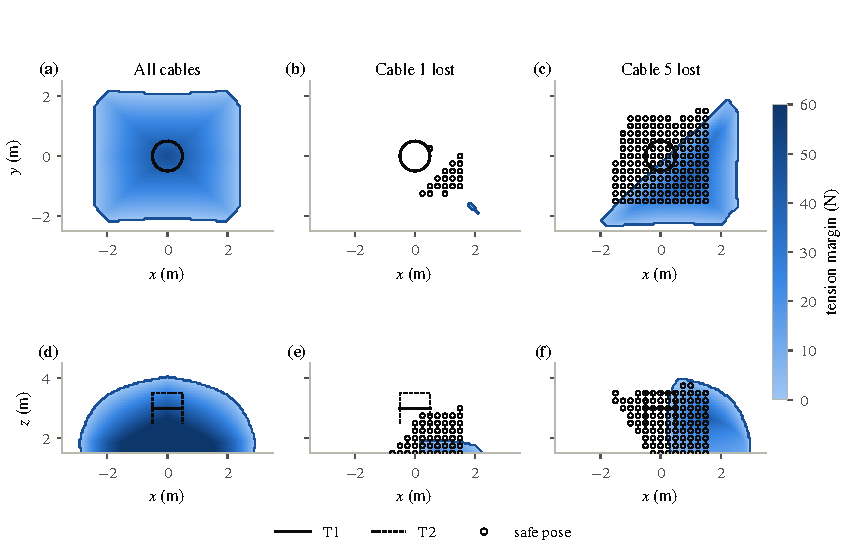
\includegraphics{fig02_postfault_workspace}
\caption{Static workspace of the level platform with all cables and after the loss of an upper or a lower cable.}\label{fig:workspace}
\end{figure}

The robot keeps more of its workspace when the platform may give up its orientation. Allowing a tilt of up to $20^\circ$ about each axis, 52.3\% of the positions can be held after an upper cable breaks and 73.8\% after a lower one, with a median tilt of $10^\circ$; the circles of Fig.~\ref{fig:workspace} mark the poses of each plane that the remaining cables then hold with a margin of at least 10~N, the targets of the recovery plans. Tilting is therefore the main resource the robot has left after a break. Redistributing the tensions and carrying on is not an option, since for most of the workspace there is no distribution to carry on with; the platform has to be moved and tilted into the feasible set of the cables that remain, and the motion has to start before that set is out of reach.

The two reference paths of the evaluation lie in the centre of the workspace (Fig.~\ref{fig:robot}). T1 is a horizontal circle of 0.5~m radius at $z=3$~m with a period of 4~s, followed for three turns in 16~s, and the helix T2 follows the same circle while climbing from $z=2.5$ to 3.5~m. The peak speed of 0.79~m/s is a third of the speed limit of the robot. On neither path can the level platform be held at any point after an upper cable breaks, while after a lower cable breaks it can on 29 to 52\% of the path, depending on the cable. An upper cable break therefore always forces the platform to leave its orientation, and a lower cable break sometimes leaves the task possible at a lower speed.

% =====================================================================
\section{Fault diagnosis}\label{sec:diagnosis}

The diagnosis has to tell eight cable breaks and eight actuator faults apart from the encoders and motor currents, and it has to do it in a few tens of milliseconds. It works on two levels because the two kinds of fault leave their signatures in different places.

\subsection{Tension estimation at each winch}\label{sec:eso}

Writing \eqref{eq:winch} with \eqref{eq:fault} as $\ddot\theta_i=b_0\tau_i+d_i$ with $b_0=1/I_m$ gathers everything that is not the commanded torque into one unknown, $d_i=-(r_dt_i+\rho_i\tau_i-f_i)/I_m$. An extended state observer \citep{han2009pid} treats $d_i$ as a third state and estimates it from the encoder,
\begin{equation}\label{eq:eso}
\begin{aligned}
\dot z_{1,i}&=z_{2,i}+3\omega_o(\tilde\theta_i-z_{1,i}),\\
\dot z_{2,i}&=z_{3,i}+b_0\tau_i+3\omega_o^2(\tilde\theta_i-z_{1,i}),\\
\dot z_{3,i}&=\omega_o^3(\tilde\theta_i-z_{1,i}),
\end{aligned}
\end{equation}
with all observer poles at $-\omega_o$, and the tension estimate is $\hat t_i=-I_m z_{3,i}/r_d$. For a bounded rate of $d_i$ the error of such an observer is ultimately bounded, with a bound that shrinks as $\omega_o$ grows \citep{guo2011eso}, but $\omega_o$ cannot grow freely, because the third channel amplifies the encoder quantisation by $\omega_o^3$. With $\omega_o=2\pi\cdot50$~rad/s the estimate followed the cable tension of the plant with an RMS error of 0.30~N at the nominal current noise and 0.57~N at twice that noise, at the price of a lag of $3/\omega_o=9.5$~ms. Comparing $d_i$ with $z_{3,i}$, the estimate converges to
\begin{equation}\label{eq:bias}
\hat t_i\ \to\ t_i+\frac{\rho_i\tau_i-f_i}{r_d}.
\end{equation}
This relation is the reason the diagnosis needs two levels. A cable break is seen at the winch, because $t_i$, and with it $\hat t_i$, drops to zero while the commanded tension does not. An actuator fault is not seen there, because it adds to $\hat t_i$ exactly the torque the motor failed to deliver: a tension loop closed on $\hat t_i$ holds the estimate at its reference while the true tension is lower by the deficit $\delta_i=(\rho_i\tau_i-f_i)/r_d$. The deficit acts on the platform, and the platform is where it has to be found. Each winch tracks the tension $t_{d,i}$ requested by the controller with
\begin{equation}\label{eq:loop}
\tau_i=r_dt_{d,i}+I_m\ddot\theta_i^{\,\mathrm{ff}}+r_d\Big(k_Pe_i+k_I\!\int e_i\,dt\Big),\qquad e_i=t_{d,i}-\hat t_i,
\end{equation}
where $\ddot\theta_i^{\,\mathrm{ff}}$ is the drum acceleration implied by the motion the controller predicts.

\subsection{Interacting multiple model estimator}\label{sec:imm}

The platform level diagnosis runs an IMM estimator \citep{blom1988imm} over the $N=2n+1=17$ modes $\mathcal M_0$ (healthy), $\mathcal B_i$ (break of cable $i$) and $\mathcal A_i$ (actuator fault of winch $i$). Each mode states which tensions the platform receives for a commanded vector $\vc t_d$,
\begin{equation}\label{eq:modes}
\vc t^{(0)}=\vc t_d,\qquad \vc t^{(\mathcal B_i)}=(\eye-\vc e_i\vc e_i^\top)\vc t_d,\qquad \vc t^{(\mathcal A_i)}=\vc t_d-\vc e_i\delta_i,
\end{equation}
where $\delta_i$ is the unknown deficit of \eqref{eq:bias}. The mode $\mathcal A_i$ merges the loss of effectiveness and the bias, because both produce the same signature at the platform. Every filter carries the state $\vc x=[\vc q^\top,\vc\nu^\top,\delta,\vc w_b^\top,\vc\eta^\top,\gamma]^\top\in\mathbb R^{28}$. The deficit $\delta$ is a random walk used only by the modes $\mathcal A_i$. The other three groups describe what the nominal model gets wrong and are shared by all modes: $\vc w_b$ is a slowly varying wrench that absorbs the errors in mass, centre of mass and inertia, $\vc\eta$ holds offsets of the length readings that absorb the errors of the anchors and of the homing, and $\gamma$ is the ratio of the true to the nominal axial stiffness. They are needed because the deficit of a mode $\mathcal A_i$ is a free parameter: without them, on a randomised plant, the filters of the actuator modes absorbed the model mismatch and won in fault free runs. A fault, in contrast, is an abrupt change that the slow bias states cannot follow on the time scale of the diagnosis, so it remains for the fault modes to explain.

Each filter propagates the mean of \eqref{eq:NE}, with its own $\vc t^{(j)}$ and the wrench $\vc w_b$ added, over the period $\Delta_I=5$~ms by a fourth order Runge--Kutta step, and the covariance with the Jacobian obtained by algorithmic differentiation. The measurement is $\vc y=[\tilde{\vc l}_u^\top,\hat{\vc t}^\top]^\top$, the unstretched lengths read from the encoders and the tension estimates of the winches, and under mode $j$ its expected value is
\begin{equation}\label{eq:h}
\tilde l_{u,i}=\frac{\gamma EA\,l_i(\vc q)}{\gamma EA+t_i^{(j)}}+\eta_i,\qquad
\hat t_i=\begin{cases}0,&j=\mathcal B_i,\\ t_{d,i},&\text{otherwise},\end{cases}
\end{equation}
where the first relation is \eqref{eq:tension} solved for the free length and the second states that the tension loop holds $\hat t_i$ at its reference unless the cable has gone. The filters take the tension commands, averaged over the period, as their input rather than the tension estimates, which lag the true tensions by 9.5~ms; this also gives the IMM a model of the motion the controller itself produces. During the first 2~s the fault modes receive no prior probability, which gives the bias states time to converge at the start of the task. The predicted probabilities are bounded below by $10^{-300}$ to keep their logarithms finite, so a fault mode can still win in that interval, but only when the healthy filter misses the measurements by an extreme margin; this happened in no run of the evaluation and in most runs of the latency study of Section~\ref{sec:latency}.

Let $\pi_{lj}$ be the probability of switching from mode $l$ to mode $j$ in one period and $\mu_l$ the mode probabilities after the previous period. One cycle computes the predicted probabilities and the mixing weights,
\begin{equation}\label{eq:mix}
\bar c_j=\sum_l\pi_{lj}\mu_l,\qquad\mu_{l|j}=\pi_{lj}\mu_l/\bar c_j,
\end{equation}
mixes the states that all filters share, runs the extended Kalman prediction and update of each filter, and obtains its innovation $\vc r^{(j)}$ with covariance $\mt S^{(j)}$. The likelihood of mode $j$ is the Gaussian density of its innovation, and the probabilities follow from Bayes' rule,
\begin{equation}\label{eq:mu}
\begin{gathered}
\ln\Lambda^{(j)}=-\tfrac12\big(\vc r^{(j)\top}\mt S^{(j)-1}\vc r^{(j)}+\ln\det(2\pi\mt S^{(j)})\big),\\
\mu_j=\frac{\Lambda^{(j)}\bar c_j}{\sum_l\Lambda^{(l)}\bar c_l}.
\end{gathered}
\end{equation}
We evaluate \eqref{eq:mu} in the log domain, subtracting the largest $\ln\Lambda^{(l)}+\ln\bar c_l$ before exponentiating. A cable break produces innovations of tens of newtons, the densities of all modes then underflow in double precision, and a direct evaluation returns $0/0$ or falls back on the prior, after which the probabilities only follow the Markov chain. In the log domain $\mu_j\ge0$ and $\sum_j\mu_j=1$ hold at every step, and the code asserts both. A fault is declared when one mode $j\ne0$ holds $\mu_j\ge\mu_{\mathrm{iso}}$ for $N_c$ consecutive cycles. The noise levels, the switching rates and the pair $\mu_{\mathrm{iso}}=0.9999$, $N_c=2$ are listed in Table~\ref{tab:settings}, with those chosen on calibration runs marked.

\begin{table}
\tbl{Settings of the estimators and the controller. Design: chosen and stated, not tuned; calibrated: chosen on calibration runs by rules written before those runs.}
{\begin{tabular}{@{}>{\raggedright\arraybackslash}p{0.17\textwidth}>{\raggedright\arraybackslash}p{0.33\textwidth}>{\raggedright\arraybackslash}p{0.24\textwidth}>{\raggedright\arraybackslash}p{0.18\textwidth}@{}}
\toprule
Part & Setting & Value & Source\\
\midrule
Winch observer and loop & bandwidth $\omega_o/2\pi$; $k_P$, $k_I$ & 50~Hz; 0.5, 20~s$^{-1}$ & design\\
IMM & period; arming time & 5~ms; 2~s & design\\
 & process noise, linear and angular acceleration & 0.5~m\,s$^{-2}$, 1~rad\,s$^{-2}$ & design; calibrated\\
 & measurement noise, lengths and tensions & 0.2~mm, 1.5~N & design\\
 & deficit random walk; fault and return rates & 20~N\,s$^{-1/2}$; $10^{-3}$, $10^{-2}$~s$^{-1}$ & design\\
Declaration & $\mu_{\mathrm{iso}}$, $N_c$ & 0.9999, 2 & calibrated\\
MPC & period, horizon & 20~ms, 12 steps & design\\
 & weights: pose; velocity; tension change & $4\times10^4$; 120; 0.03 & calibrated\\
 & after a break declaration & velocity $\times0.3$, tension change $\times3$ & calibrated\\
 & scenarios: threshold $\mu_s$, at most & $10^{-3}$, 2 fault scenarios & design\\
Planner & time scaling: horizon, $\kappa_{\min}$ & 2~s, 0.25 & design\\
 & recovery \eqref{eq:recovery}: $T$, intervals; $s_p$, $s_{\min}$ & 1~s, 15; 5, 10~N & design\\
 & library: break instants; detection delay & every 50~ms; 15~ms & design\\
\bottomrule
\end{tabular}}
\label{tab:settings}
\end{table}

% =====================================================================
\section{Control and recovery}\label{sec:control}

Fig.~\ref{fig:architecture} shows how the parts fit together: the observers give the IMM the winch tensions, the IMM gives the MPC the mode probabilities, the platform state and the deficit of a faulty winch, and the dashed lines mark the fault scenarios that the MPC can weight before a declaration. Algorithm~\ref{alg:cycle} gives the order in which the parts run.

\begin{figure}
\centering
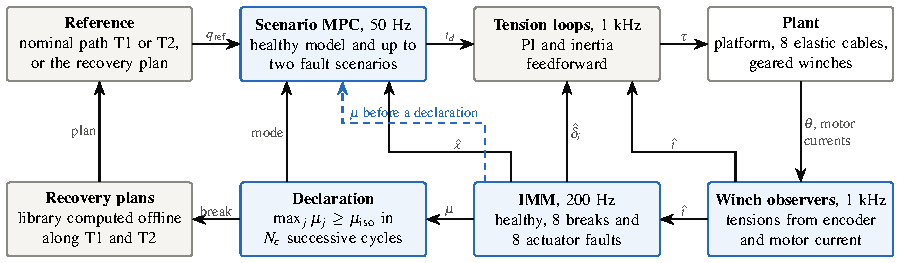
\includegraphics[width=\textwidth]{fig03_architecture}
\caption{Structure of the fault tolerant controller.}\label{fig:architecture}
\end{figure}

\begin{algorithm}
\caption{One cycle of the controller}\label{alg:cycle}
\small
\begin{algorithmic}[1]
\Require read the encoder angles and motor torques of the previous sample
\State update the observer \eqref{eq:eso} of every winch; $\hat t_i\gets-I_mz_{3,i}/r_d-\hat\delta_i$ if winch $i$ is declared faulty
\If{5~ms have passed since the last IMM cycle}
  \State run the IMM \eqref{eq:mix}--\eqref{eq:mu} with the averaged commands; obtain $\vc\mu$, $\hat{\vc x}$, $\hat\delta_i$
  \If{no fault is declared and $\mu_j\ge\mu_{\mathrm{iso}}$ in $N_c$ cycles for one $j\ne0$}
    \State declare $j$; the MPC predicts with mode $j$ from now on
    \If{$j=\mathcal B_i$} \State take the plan of cable $i$ for the instant nearest $t-15$~ms; scale the MPC weights \EndIf
  \EndIf
\EndIf
\If{20~ms have passed since the last MPC solve}
  \State solve \eqref{eq:mpc} from $\hat{\vc x}$ (scenarios from $\vc\mu$ before a declaration); obtain $\vc t_d$, $\ddot{\vc\theta}^{\,\mathrm{ff}}$
\EndIf
\State apply the tension loop \eqref{eq:loop} of every winch
\end{algorithmic}
\end{algorithm}

\subsection{Model predictive control with fault scenarios}\label{sec:mpc}

At each control instant the scenario set $\mathcal J=\{0\}\cup\{j:\mu_j\ge\mu_s\}$ holds the healthy mode and the fault modes whose probability exceeds $\mu_s=10^{-3}$, at most the two most probable ones, with weights $\tilde\mu_j=\mu_j/\sum_{l\in\mathcal J}\mu_l$. The controller solves
\begin{equation}\label{eq:mpc}
\begin{aligned}
\min_{\vc t_0,\dots,\vc t_{N-1}}\ &\sum_{j\in\mathcal J}\tilde\mu_j\Big[\sum_{k=0}^{N-1}\big(\lVert\vc x^{(j)}_k-\vc x^{\mathrm{ref}}_k\rVert^2_{\mt Q_x}+\lVert\vc t_k-\vc t_{k-1}\rVert^2_{\mt Q_t}\big)\\
&\qquad\quad+V_f^{(j)}(\vc x^{(j)}_N)\Big]\\
\text{s.t.}\ &\vc x^{(j)}_{k+1}=\vc f_d\big(\vc x^{(j)}_k,\vc t^{(j)}(\vc t_k)\big),\quad\vc x^{(j)}_0=\hat{\vc x}^{(j)},\\
&t_{\min}\le t_{k,i}\le t_{\max},\qquad j\in\mathcal J,
\end{aligned}
\end{equation}
where $\vc x^{(j)}_k=(\vc q,\vc\nu)$ is the platform state predicted under mode $j$, $\vc f_d$ is \eqref{eq:NE} discretised over the control period and $\vc t^{(j)}(\cdot)$ the map \eqref{eq:modes}. All scenarios share one tension sequence, so the first command suits every mode that is still plausible. For the healthy mode the terminal cost $V_f^{(0)}$ penalises the distance to the reference; for a fault mode it pulls the predicted pose toward the nearest pose that the remaining cables hold with a margin of 10~N, looked up from sets stored offline. As $\mu_j$ grows, this term starts moving the platform toward the region in which it would survive fault $j$ before the fault is confirmed; we call this the probability weighting of the scenarios. The probabilities weight costs only: the tension bounds are the same box for every scenario and do not depend on them. \citet{raman2023cable} used IMM weights to blend the outputs of mode specific controllers, whereas in \eqref{eq:mpc} the probabilities weight predicted costs inside one optimisation, so the tension bounds hold whichever mode is true. With the healthy mode alone, \eqref{eq:mpc} is a tracking MPC with tension bounds whose first command also solves the tension distribution problem. In the implementation the predictions also carry the bias wrench $\hat{\vc w}_b$ of the IMM, the stage cost of a fault scenario is scaled by 0.1, and two small terms are added, a pull toward the feedforward tensions of the reference and a penalty on predicted free lengths that approach the ends of their drum windows; the complete formulation is in the repository.

The horizon is $N=12$ steps of 20~ms. The programme is written in CasADi \citep{andersson2019casadi} and solved by IPOPT \citep{wachter2006ipopt} with the exact Hessian, warm started from the shifted previous solution. After a break declaration the velocity weights are scaled down and the weight of the tension changes up (Table~\ref{tab:settings}), because the elasticity of the cables, which the prediction model leaves out, matters more with seven cables: at the end poses of the recovery plans the lowest elastic mode of the platform falls to 3.2 to 3.6~Hz, against 5.5~Hz at the home pose with eight cables. We do not claim recursive feasibility or closed loop stability for \eqref{eq:mpc}. The plant differs from the prediction model through the cable elasticity, the winch dynamics and the estimation errors, and the scenario set changes with time. The tension box itself never becomes infeasible, since it does not depend on the state; what can be lost is the ability to track, and the evaluation measures it instead of assuming it. The bounds apply to the tension commands. The tensions of the elastic cables in the plant follow the commands through the tension loops and can leave the bounds, and the evaluation measures them in the plant, for the intact cables only. When IPOPT returns without success, the controller applies the iterate it returns, with the commands clipped to their bounds; no fallback is used. All 399 unsuccessful solves of the evaluation stopped at the limit of 30 iterations (Appendix~\ref{sec:replay}).

\subsection{Accommodation of actuator faults}\label{sec:accommodation}

After the declaration of an actuator fault $\mathcal A_i$ the reference is kept, and the tension loop of winch $i$ is corrected by the deficit that the filter of the declared mode estimates, $\hat t_i\leftarrow\hat t_i-\hat\delta_i$ in \eqref{eq:loop}. After a break declaration the winch of the broken cable is held at its angle, so that it does not run away once its load is gone.

\subsection{Recovery plan}\label{sec:planner}

Once a break of cable $i$ is declared, the planner decides what the platform can still do, in two branches tried in order. In the first, time scaling, the remaining reference over the next 2~s is slowed down by the largest factor $\kappa\in[0.25,1]$ for which the margin \eqref{eq:margin}, with the inertial wrench of the slowed motion added to gravity, stays nonnegative at every sample with the seven cables. Below $\kappa=0.25$ the task no longer continues in any useful sense, and the second branch, recovery, brings the platform to rest within $T=1$~s at a pose the remaining cables hold with a margin of $s_{\min}=10$~N. The recovery path solves an optimal control problem on the rigid model with the remaining cables,
\begin{equation}\label{eq:recovery}
\begin{aligned}
\min\ &\lVert\vc q_N-\hat{\vc q}\rVert^2_{\mt Q_q}+h\sum_k w_v\lVert\vc\nu_k\rVert^2+h\sum_k w_a\Big\lVert\frac{\vc\nu_{k+1}-\vc\nu_k}{h}\Big\rVert^2\\
&+w_r\sum_k\lVert\vc t_{k+1}-\vc t_k\rVert^2+w_s\sum_k s_k\\
\text{s.t.}\ &\vc x_0=\hat{\vc x},\ \ \text{collocation of \eqref{eq:NE} on every interval},\\
&t_{k,i}=0,\quad t_{\min}+s_p-s_k\le t_{k,l}\le t_{\max}-s_p+s_k,\ \ l\ne i,\\
&s_k\ge0,\quad\lVert\dot{\vc p}_k\rVert\le v_{\max},\quad\lVert\vc\varphi_k\rVert_\infty\le25^\circ,\quad\vc\nu_N=\vc0,\\
&\mt W(\vc q_N)\vc t_{\mathrm{hold}}+\vc w_g(\vc q_N)=\vc 0,\quad\lVert\vc\varphi_N\rVert_\infty\le20^\circ,\\
&t_{\min}+s_{\min}\le t_{\mathrm{hold},l}\le t_{\max}-s_{\min},\ \ l\ne i,
\end{aligned}
\end{equation}
transcribed by Hermite--Simpson collocation \citep{kelly2017collocation} on 15 intervals of $h=T/15$ with the tensions constant over each, and solved with IPOPT. The terminal conditions say that the platform ends at rest at a pose the remaining cables hold, and the first term picks among those poses one close to the pose at the break. The twist and acceleration terms keep the motion direct and smooth, and the margin $s_p=5$~N is relaxed by slacks $s_k$, which widen the admissible tension region. The dynamics, the attitude, speed and acceleration limits, the drum windows and the rest at the end remain hard constraints, so the slacks do not make the problem feasible from an arbitrary state. A solution with nonzero slacks would mark a third branch, a descent with the least violation of the tension bounds. Three constraints of the implementation are left out of \eqref{eq:recovery} for clarity: a soft tension margin of 20~N, penalised quadratically, which keeps tension in reserve for the feedback of the MPC, the acceleration limit of Table~\ref{tab:parameters}, and the drum windows of the remaining cables.

\label{sec:library}Solving \eqref{eq:recovery} took 0.21~s in the median and at most 0.82~s on one core, and the platform falls during that time. Because the reference paths of a task are known before the task runs, the planner is therefore evaluated in advance. For each path and each cable, the branch and the plan are computed for break instants every 50~ms from 2.5 to 8.0~s, which covers the possible onsets with room for the detection delay. On a declaration at $t_d$ the controller takes the plan of the instant nearest to $t_d-15$~ms, the typical delay of a break declaration, and passes it to the MPC as the new reference together with its tensions as feedforward. Every plan after an upper cable break needed the recovery branch, with a median drop of the reference point of 0.54 to 0.60~m depending on the cable, whereas after a lower cable break the time scaling sufficed for 31 to 69 of the 222 instants of both paths and the recovery plans dropped by at most 0.02~m. The platform hanging from seven cables is unstable along these paths: integrated in open loop with the plan's tensions, it drifts from a recovery path after an upper cable break by up to 0.11~m by its end, so the plan has to be tracked in closed loop. All 1,605 recovery problems of the library met the termination criteria of IPOPT, 1,603 at its optimal and 2 at its acceptable level, with every slack zero, so every plan satisfies the tension margins with the tensions it holds over each interval; integrated again interval by interval on the rigid model, the plans deviate from their collocation solution by at most 0.12~mm. This is evidence for the sampled break instants on the rigid model, not a guarantee for other states or for the elastic plant, on which the evaluation tests the plans in closed loop.

% =====================================================================
\section{Evaluation}\label{sec:evaluation}

\subsection{Simulator}\label{sec:simulator}

The simulator integrates the full model of Section~\ref{sec:model}: the rigid platform with its orientation as a unit quaternion, eight elastic unilateral cables \eqref{eq:tension} and eight winches \eqref{eq:winch} with the torque and speed limits of their drives. At every millisecond it switches on a fault whose onset has been reached, reads the sensors, hands the controller the reading of the previous sample and integrates the plant over the millisecond in 16 Runge--Kutta steps of 62.5~$\mu$s, a step fixed by a convergence test. The plant was verified against a stiff reference solution and against an independent model in MuJoCo \citep{todorov2012mujoco} (Appendix~\ref{app:verification}). The controller never reads the plant state, and it uses the nominal parameters and the rigid model \eqref{eq:NE}; the gap between plant and prediction model is the one any model based controller meets on a real robot, and keeping it prevents the controller from being tested against its own design model. A run counts as a lost platform, and stops, when one of the three attitude angles (roll, pitch or yaw) exceeds $30^\circ$, when $P$ leaves the interior of the frame, or when the drum of an intact cable leaves its window. The rule on the attitude includes yaw, which is not an inclination; Appendix~\ref{sec:replay} reports which losses it decided on yaw alone and what a rule on roll and pitch alone would change.

Every setting of every method was fixed on calibration runs that share no parameter draw, noise sequence or fault onset with the evaluation, and the protocol of the evaluation, with its methods, runs, endpoints and statistics, was written before any evaluation run. It was amended once: the first evaluation runs showed that the gains of the threshold baseline had been chosen by a rule that ignored the tension bounds, so its settings were chosen again on calibration runs and the evaluation was restarted from its first run, with no setting of any other method changed.

\subsection{Methods compared}\label{sec:methods}

Table~\ref{tab:methods} lists the nine methods that we tested and compared. The ablations A1, A2 and A3 remove one part of the proposed controller P each: the probability weighting of the scenarios, the replanning after a break, and the library, whose plan A3 solves online and applies after a latency of 0.4~s, which covers the 99th percentile of the solve times. B0 has no fault tolerance, and the oracle B1 is told the true fault at its onset, which bounds what a perfect diagnosis would achieve with the same controller.

% written by scripts/paper_tables.py from stored files; do not edit
\begin{table}
\tbl{Methods of the evaluation.}
{\begin{tabular}{@{}lp{0.8\linewidth}@{}}
\toprule
Method & Description \\
\midrule
P & Proposed: IMM diagnosis; before a declaration the MPC weights the fault scenarios by their probabilities; after a break declaration it follows a plan from the library \\
A1 & P without the probability weighting of the scenarios \\
A2 & P without replanning after a break \\
A3 & P with the recovery plan solved online, applied after 0.4~s \\
B0 & No fault tolerance: healthy model throughout, no declaration \\
B1 & Oracle: the true fault declared at its onset \\
B2 & Thresholds on the winch tension estimates, computed torque control with tension distribution, plans from the library \\
B3 & Recurrent classifier in place of the IMM probabilities for the declaration; A1 otherwise \\
B3T & B3 with the classifier probabilities also weighting the MPC scenarios \\
\bottomrule
\end{tabular}}
\label{tab:methods}
\end{table}


The threshold baseline B2 stands for the classical pipeline: thresholds on the winch quantities for the diagnosis, a computed torque law with the tension distribution \eqref{eq:margin} instead of the MPC, and the same plan library as P. Its gains and thresholds were chosen on calibration runs of its own controller. It declares a break when the tension estimate of a winch falls below 9~N. Every threshold on the tension residual that detected an actuator fault also raised false alarms with this controller, so B2 does not isolate actuator faults; it is a break detector, which is what the classical literature on cable robots offers.

The learned baseline B3 replaces the mode probabilities of the IMM by those of a recurrent classifier for the declaration, while the filters of the IMM keep running as the state estimator, so that B3 differs from A1 in the diagnosis alone. In B3T the classifier's probabilities also weight the fault scenarios of the MPC, as the IMM's do in P. The classifier has the same seventeen classes as the IMM and sees the same information: at every estimator cycle, the tension residual $\hat t_i-t_{d,i}$, the tension estimate $\hat t_i$ and the deviation of the free length from its value at the reference pose, for each winch. A long short term memory network \citep{hochreiter1997lstm} of two layers of 64 units reads the last 0.1~s of these 24 channels; its architecture and hyperparameters came from a search of 30 trials on validation runs \citep{akiba2019optuna}. It was trained on 528 runs of both paths, recorded with the controller without the weighting and with declarations disabled, so that the motion carries no trace of any diagnosis. Its outputs were calibrated by temperature scaling \citep{guo2017calibration}, and the declaration rule of the IMM was applied to them with thresholds chosen on validation runs.

\subsection{Runs, metrics and statistics}\label{sec:protocol}

Every fault type was injected on every cable of both paths in 13 repetitions: a break, a loss of effectiveness of $\rho=0.3$ or 0.6, and a torque bias of $\pm10\%$ of the holding torque, the two values of $\rho$ and the two signs of the bias alternating over the repetitions: $2\times3\times8\times13=624$ fault runs, 208 of each type, with the onset drawn uniformly between 3 and 7~s and the run ending 4~s after it or when the platform is lost. There were 100 fault free runs of 16~s per path. Each run draws its plant parameters from its seed (Table~\ref{tab:parameters}), and the current noise is nominal in half of the runs and doubled in the other half. All methods ran on the same seeds, so every comparison is paired. Counting every method on every run it applies to, B3T on a subset fixed in advance, the evaluation comprises 5,212 simulations.

Errors are taken to the active reference, the nominal path before a declaration and the plan after it, and the transient is the 2~s after the onset. The diagnosis is scored by the declared mode, its delay and the false alarms, declarations before the onset or in a fault free run counted per hour of operation with the fault modes armed. The recovery time is the time from the onset after which the position error stays for 1~s within twice the 95th percentile of the error in the fault free runs of the same path. Six primary endpoints were fixed with their comparisons, each with a Holm correction: the platform lost after a break, the fault declared with the correct mode, the delay of the correct declarations, the false alarms per hour, the smallest tension margin in the transient and the share of the transient outside the bounds. Shares carry 95\% Wilson intervals and paired comparisons McNemar's exact test; continuous endpoints are compared with the Wilcoxon signed rank test and bootstrap intervals. No run was excluded.

% =====================================================================
\section{Results}\label{sec:results}

Table~\ref{tab:results} gives the outcome of every method; A2 and A3 ran the break runs only and B3T a subset fixed in advance, and the complete statistics of the six endpoints are in the repository given under Data availability.

% written by scripts/paper_tables.py from stored files; do not edit
\begin{table}
\tbl{Outcome of every method in the evaluation.}
{\begin{tabular}{@{}lrrrrrr@{}}
\toprule
& \multicolumn{2}{c}{Lost in break runs} & Correct & Median break & False alarms & Breaks \\
\cmidrule(lr){2-3}
Method & upper & lower & declarations & delay (ms) & (per h) & recovered \\
\midrule
P & 11/104 & 0/104 & 623/624 & 17 & 0.8 & 181/208 \\
A1 & 11/104 & 0/104 & 624/624 & 17 & 0.0 & 182/208 \\
A2 & 31/104 & 7/104 & 208/208 & 17 & -- & 74/208 \\
A3 & 20/104 & 0/104 & 208/208 & 17 & -- & 173/208 \\
B0 & 104/104 & 18/104 & -- & -- & -- & 0/208 \\
B1 & 3/104 & 1/104 & 624/624 & -- & -- & 197/208 \\
B2 & 35/104 & 30/104 & 208/624 & 22 & 3.1 & 93/208 \\
B3 & 24/104 & 1/104 & 598/624 & 30 & 32.5 & 157/208 \\
B3T & 28/32 & 16/32 & 16/192 & 532 & 505.1 & 19/64 \\
\bottomrule
\end{tabular}}
\label{tab:results}
\end{table}


\subsection{One break in detail}\label{sec:example}

Fig.~\ref{fig:example} follows one break, chosen by a rule fixed before drawing: among the upper cable breaks whose traces were kept, the run with the median declaration delay of P. Cable~2 breaks at 4.933~s on T1. The IMM gives the break mode a probability above 0.99 in the cycle 11~ms after the break and declares it after 17~ms. The classifier's probability rises earlier, to 0.99 at 6~ms, but both reach the threshold of 0.9999 in the same cycle, 11~ms after the break; the IMM needs two such cycles and declares after 17~ms, the classifier needs four and declares after 27~ms, and the threshold rule of B2 declares at 22~ms. The platform cannot stay where it is. Under P it descends by 0.5~m along the recovery plan to a pose the seven remaining cables can hold, tilting by at most $6.7^\circ$ and settling at $5.3^\circ$, while the seven intact cables take over the load of cable~2: an intact cable leaves its bounds for 5\% of the first 2~s, all of it within 0.21~s of the break, and from 0.3~s on every intact tension lies between 15 and 183~N. Without fault tolerance the platform turns past $30^\circ$ and is lost 0.40~s after the break. Fig.~\ref{fig:example} shows (a) the probability of the true mode up to the declarations (vertical lines), (b) the height with the recovery plan, (c) the tilt of the platform axis from the vertical, with a cross where the roll of B0 passes $30^\circ$, and (d) the plant tensions under P against the bounds of the tension commands; the curves of B3 lie under those of P.

\begin{figure}
\centering
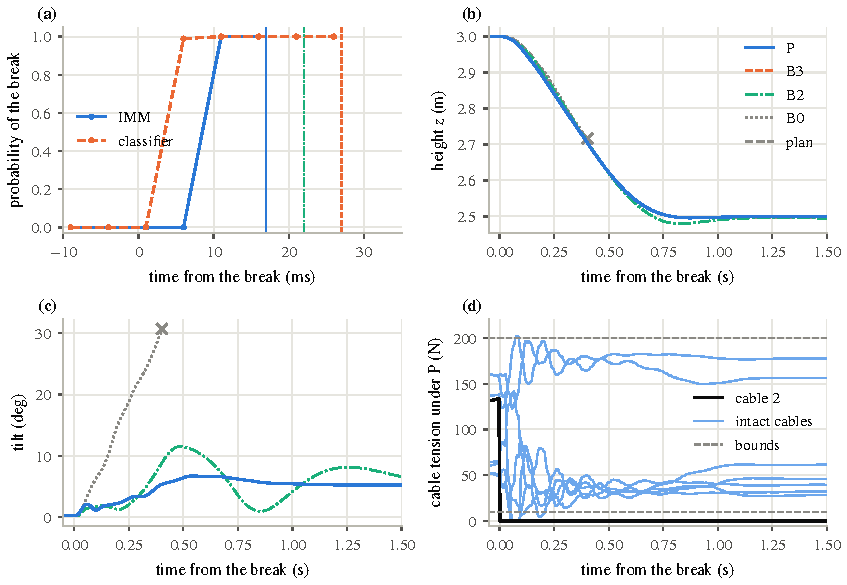
\includegraphics{fig04_example_break}
\caption{Response to a break of the upper cable~2 at 4.933~s on T1 (run~1 of the evaluation).}\label{fig:example}
\end{figure}

\subsection{Detection and isolation}\label{sec:detection}

The IMM declared 623 of the 624 faults with the correct mode (Fig.~\ref{fig:delays}). Its median delay was 17~ms for a break, 23~ms for a loss of effectiveness and 41~ms for a bias, and no break took longer than 19~ms. Its one false alarm, 2.8~s before a loss of effectiveness of the same winch, is also the one fault it did not declare correctly. On the same runs P declared 5~ms earlier than B2 and 10~ms earlier than B3 (paired medians). B2 declared every break correctly and no actuator fault, and in 21 runs with a loss of effectiveness of an upper winch it declared a break of a healthy lower cable whose tension had fallen below its threshold. The classifier of B3 declared all 208 breaks correctly, 206 of the 208 losses of effectiveness and 184 of the 208 biases. Each curve of Fig.~\ref{fig:delays} covers the 208 runs of one fault type and ends at the share declared correctly.

\begin{figure}
\centering
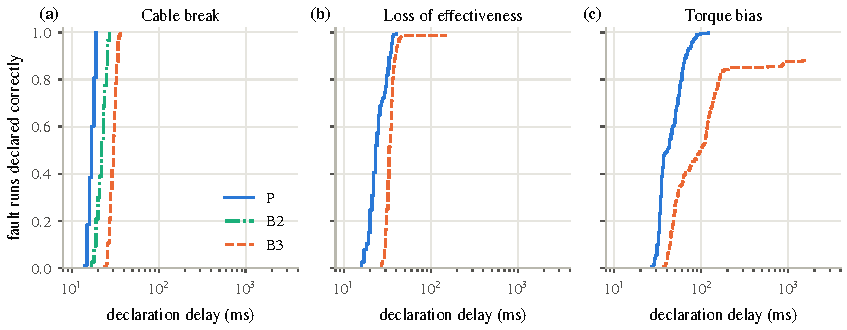
\includegraphics{fig05_detection_delay}
\caption{Fault runs declared with the correct mode within a given delay after the onset.}\label{fig:delays}
\end{figure}

The difference that matters most in closed loop is the false alarm. The classifier raised 42 false alarms in the 1.29~h of operation in which P raised one, and its fault free runs carried a false alarm in 4 of 100 on T1 and in 34 of 100 on T2 (Fig.~\ref{fig:falsealarms}, where B3T has 30 fault free runs per path); the IMM raised none there, with or without the weighting. Training on both paths brought its isolation close to that of the IMM, but not its rate of false alarms on the helix (Fig.~\ref{fig:learned}). The offline results of that figure are single tests on the same stored runs, 8 fault free and 80 fault runs per path, of the classifier trained on T1, of the classifier trained on both paths and of the IMM; the closed loop results are those of the evaluation. A first classifier trained on T1 alone had shown how strongly the learned diagnosis depends on its training data: on the helix it raised a false alarm in 6 of 8 fault free test runs and declared 45 of 80 faults correctly, taking the healthy motion along the climbing path for actuator faults of the lower winches, while the IMM, which uses a model of the robot rather than examples of its motion, kept its performance on both paths.

\begin{figure}
\centering
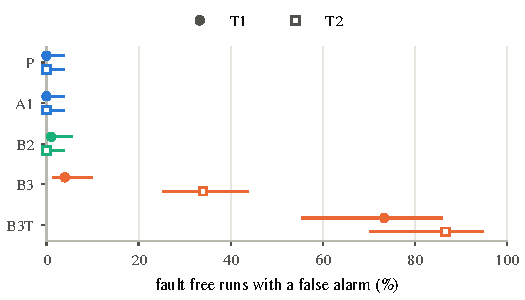
\includegraphics{fig06_false_alarms}
\caption{Fault free runs with a false alarm, with 95\% Wilson intervals.}\label{fig:falsealarms}
\end{figure}

\begin{figure}
\centering
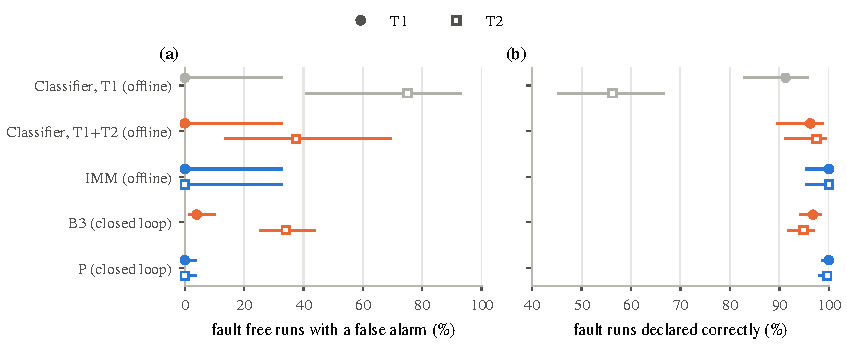
\includegraphics{fig07_learned_vs_model}
\caption{Learned against model based diagnosis, offline and in closed loop, with 95\% Wilson intervals: (a) fault free runs with a false alarm; (b) fault runs declared with the correct mode.}\label{fig:learned}
\end{figure}

\subsection{Safety after a break}\label{sec:safety}

The proposed controller lost the platform after 11 of the 208 breaks (5.3\%), against 122 without fault tolerance (58.7\%), 65 for B2 (31.2\%), 25 for B3 (12.0\%) and 38 without replanning (18.3\%); every one of these differences remains after the Holm correction. All 11 losses of P followed the break of an upper cable, 6 of 52 on T1 and 5 of 52 on T2, and P kept the platform after every lower cable break (Fig.~\ref{fig:safety}). The oracle B1 lost 4, three of them after upper cable breaks, so even a diagnosis without delay cannot save every upper cable break with this controller. The price of the 17~ms of diagnosis appears in the tension bounds rather than in the losses: during the 2~s after a break a cable was outside its bounds for 5.1\% of the time under P and 2.1\% under the oracle (medians). B2, with its gains tuned on its own calibration runs and the same plans, lost 65 platforms, 30 of them after a lower cable break, after which P never lost one.

\begin{figure}
\centering
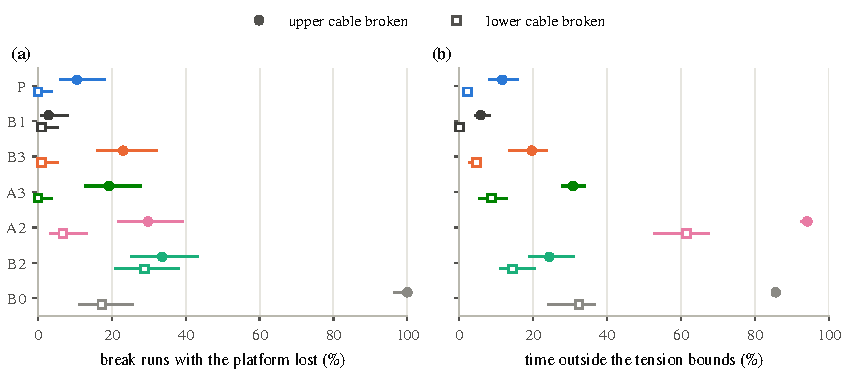
\includegraphics{fig08_safety_after_break}
\caption{Safety after the 104 upper and 104 lower cable breaks: (a) runs with the platform lost, with 95\% Wilson intervals; (b) median share of the 2~s after the break with an intact cable outside its tension bounds, with 95\% bootstrap intervals.}\label{fig:safety}
\end{figure}

\subsection{Recovery}\label{sec:recovery}

Replanning carries most of this result. Without it (A2), 38 platforms were lost, 86.5\% of the transient was spent outside the bounds in the median, and the error after the transient was 72.7~mm against 5.6~mm for P. The library matters as well: solving the plan online with its latency (A3) lost 20 platforms against 11 (paired, $p=0.09$, a secondary comparison) and raised the time outside the bounds in the transient from 5.1 to 20.2\%. With P the position error returned to the band of the fault free runs in 181 of the 208 break runs, after 0.27~s in the median (Fig.~\ref{fig:recovery}, where lost runs and runs that did not recover before their end never reach the curves); the oracle recovered 197 runs after 0.19~s, A3 173 after 0.70~s and A2 74 after 1.01~s.

\begin{figure}
\centering
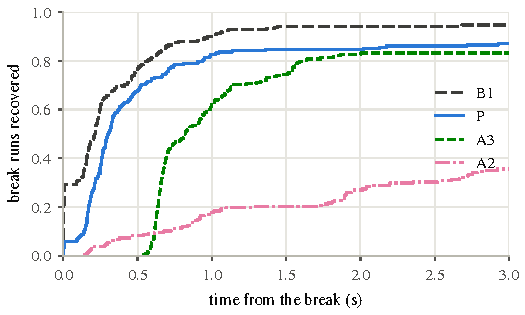
\includegraphics{fig09_recovery}
\caption{Break runs whose position error has returned to the band of the fault free runs within a given time.}\label{fig:recovery}
\end{figure}

\subsection{Actuator faults}\label{sec:actuator}

No method that isolates actuator faults lost a platform after one, except B3T, which lost 14 after the onset of an actuator fault and 37 more in such runs before the onset (Section~\ref{sec:tightening}). B2, which cannot isolate them, lost 18 platforms after a loss of effectiveness, and in three other runs with an actuator fault it lost the platform before the onset, after a false alarm. The accommodation of P is biased, however. After a loss of effectiveness, the IMM's estimate of the deficit had an RMS error of 30~N in the median, 20~N for $\rho=0.3$ and 52~N for $\rho=0.6$, and the error after the transient was 18.2~mm, 14 and 45~mm for the two magnitudes, so that only 80 of the 208 runs returned to the band of the fault free runs. After a bias the deficit error was 5.6~N and 206 of 208 runs returned to the band. The cause is the structure of the accommodation: the IMM keeps the tension commands as its input while the loop of the faulty winch is corrected by the deficit it estimates, so its filter then estimates the deficit that remains after the correction, and the pair settles at about half of the true deficit.

\subsection{The probability weighting of the scenarios}\label{sec:tightening}

With the IMM the weighting had no measurable effect on the safety endpoints; in Fig.~\ref{fig:tightening}(a) the 624 paired runs lie on the diagonal. P and A1 lost the same number of platforms after a break, 11 each, with the outcome differing in ten runs, five each way, and their tension margins in the transient did not differ (paired median difference 0~N, $p=0.26$). Their declarations differed in two respects, which a comparison of the paired runs after the evaluation showed and which the analysis plan did not include. P raised one false alarm, 2.8~s before a loss of effectiveness that A1 declared correctly, and in 51 of the 208 runs with a torque bias the two declared at different times, P earlier in 49 of them, by 5 to 15~ms, and later in two; breaks and losses of effectiveness were declared at the same times. Before a fault the weighting was almost never active: the position error before the fault was identical in 804 of the 824 paired runs. The reason is the speed with which breaks are declared. Every break was declared within 19~ms, less than the 20~ms period of the MPC, so the MPC solves at most once with intermediate probabilities before it switches to the model of the declared mode. The weighting can only act while the diagnosis is uncertain, and for a break that interval is shorter than one control period.

\begin{figure}
\centering
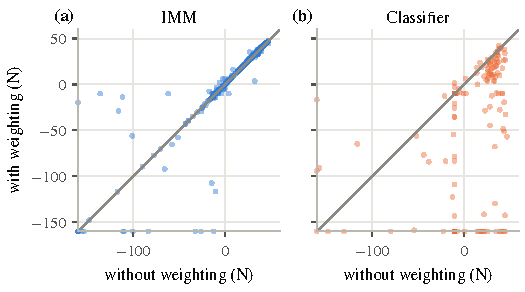
\includegraphics{fig10_tightening}
\caption{Smallest tension margin of the intact cables in the 2~s after the fault, with the weighting against without it: (a) IMM, P against A1; (b) classifier, B3T against B3.}\label{fig:tightening}
\end{figure}

With the classifier the closed loop became much worse. On the runs of B3T, with its probabilities weighting the scenarios of the MPC, a false alarm was raised in 154 of 252 runs against 11 for B3 on the same runs, the correct declarations fell from 186 to 16 of 192, the platform was lost in 44 of 64 break runs against 8, in 17 of them before the cable broke, and the margin in the transient fell by 19~N (paired median; 95\% interval $-28.7$ to $-13.8$~N). In Fig.~\ref{fig:tightening}(b) most of the 138 paired runs in which B3T reached the fault lie below the diagonal; margins below $-160$~N are drawn at $-160$~N. Unsuccessful solves of the MPC came with this. IPOPT returned without success in 382 solves in 111 of the 252 runs of B3T, against one solve in one run for P. The replay of Appendix~\ref{sec:replay} recorded every solve of the lost runs: all unsuccessful ones stopped at the limit of 30 iterations, 318 of the 335 with the healthy and two fault scenarios in the programme, and the iterates they returned violated the equality constraints of the prediction by 0.14 in the median and by up to 116 (in metres, radians or their rates), against at most 0.004 for the eight unsuccessful solves in the lost runs of A2. Of the 114 platforms B3T lost, 73 were lost before any fault, 19 of them in fault free runs; 61 of these 73 runs contained an unsuccessful solve, 22 a false declaration, and 51 no declaration at all. In each of the 78 lost runs with an unsuccessful solve the first one came before the loss, by 0.53~s in the median, and in 55 of them the attitude was still below $10^\circ$ when it came; in 33 other runs the solver failed and the platform was kept. The unsuccessful solves are therefore a plausible part of the mechanism, but these runs cannot separate how much the probabilities of the classifier, the motion the weighting produced and the convergence of the solver each contributed.

\subsection{Computation}\label{sec:compute}

The simulation waits for each solve, so the closed loop behaved as if every computation met its period. On the machine of the evaluation, with two runs sharing two cores, they did not all do so (Fig.~\ref{fig:compute}). The estimator cycle of the observers and the IMM took 2.9~ms on average and 5.3~ms at the 99th percentile, against its period of 5~ms. The MPC took 32~ms on average and 65~ms at the 99th percentile, against its period of 20~ms, so the controller as implemented, with CasADi and IPOPT and the models compiled to C, would not run in real time on this machine, and Section~\ref{sec:latency} shows that it needs its solutions on time.

\begin{figure}
\centering
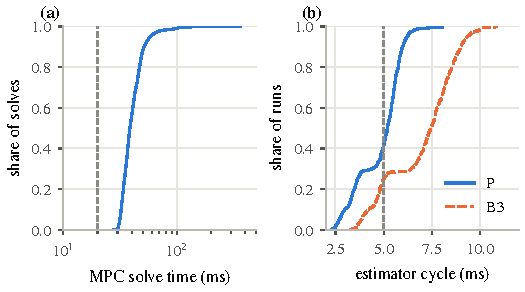
\includegraphics{fig11_computation}
\caption{Computation times against their periods: (a) every MPC solve of P in the kept fault runs; (b) 99th percentile of the estimator cycle of every run of P and of B3.}\label{fig:compute}
\end{figure}

\subsection{Sensitivity to the computation time of the MPC}\label{sec:latency}

In the evaluation every output of the MPC acted in the sample in which its solve began, although the solves took 32~ms on average (Section~\ref{sec:compute}). After the evaluation we tested what this assumption carries, under a protocol written and published before the runs. P ran again on the 104 upper cable breaks, which contain all its losses, with the output of the MPC available a fixed computation time $D$ after its solve begins. For $D>0$ a solve begins every $\max(20~\mathrm{ms},D)$ and uses the state estimate, the reference and the command applied at that instant; its first tension command and the feedforward of the drum acceleration take effect $D$ later and are held until the next solution takes effect. The observers, the IMM, the declaration and the tension loops keep their timing, and neither the controller nor its settings were changed after the results were seen. With $D=0$ all 104 rows were identical to those of the evaluation.

% written by scripts/paper_tables.py from stored files; do not edit
\begin{table}
\tbl{Sensitivity of P to the computation time $D$ of the MPC on the 104 upper cable breaks.}
{\begin{tabular}{@{}rrrrrrrrr@{}}
\toprule
$D$ & Period & Lost & 95\% CI & Lost before & $p$ & Outside & Smallest & Correct \\
(ms) & (ms) & & (\%) & the break & (Holm) & bounds (\%) & margin (N) & declarations \\
\midrule
0 & 20 & 11/104 & 6--18 & 0 & -- & 11.6 & -10 & 104/104 \\
20 & 20 & 104/104 & 96--100 & 104 & $<0.001$ & -- & -- & 0/104 \\
40 & 40 & 104/104 & 96--100 & 104 & $<0.001$ & -- & -- & 0/104 \\
60 & 60 & 104/104 & 96--100 & 104 & $<0.001$ & -- & -- & 0/104 \\
\bottomrule
\end{tabular}}
\label{tab:latency}
\end{table}


Table~\ref{tab:latency} compares every delay with $D=0$ on the same runs by the exact McNemar test, with the Holm correction over the three delays; its tension measures are medians over the runs that reached the break, which no delayed run did. The controller did not tolerate any of the delays. With the output one period late, $D=20$~ms, the platform was lost in all 104 runs, and every loss came before the cable broke, between 0.66 and 1.40~s after the start, while the breaks were due between 3 and 7~s. The roll of the platform oscillated at about 5~Hz with an amplitude that grew by a factor of 32 in the median over half a second, and every run ended on roll. In every run the IMM, not yet armed, then declared a fault of an intact cable or winch, a break of an upper cable in 100 of them, and the platform was lost 0.17 to 0.55~s later. The declaration did not start the motion, since in 77 runs roll or pitch had already passed $5^\circ$, but it may have hastened the loss; the runs do not separate the two. With 40 and 60~ms the platform was lost in every run as well, again before the break, and unsuccessful solves appeared in 68 and 55 of the runs. The largest computation time tested without significantly more losses than at $D=0$ is therefore 0~ms.

The results of this paper therefore hold for an MPC whose solution acts within its sample, not for the implementation timed in Section~\ref{sec:compute}. A fixed delay is a model of the computation time and not a real time implementation: the study shows the sensitivity to the delays tested, not whether a given computer meets them. Delays shorter than one period, and an MPC that predicts the state at the instant its command takes effect, were not tested.

% =====================================================================
\section{Discussion}\label{sec:discussion}

The IMM separates faults through what each mode predicts, and the predictions differ where the physics of Section~\ref{sec:eso} says they should. A break makes the tension estimate of one winch fall to zero while its command does not, which only the break mode of that cable explains, and this is why every break was declared within four estimator cycles. An actuator fault leaves the winch estimate at its command and moves the platform, which the length readings of all eight cables register, so the actuator modes need more evidence and take longer. The filters also take the controller's own tension commands as their input, and so they carry a model of the motion the controller produces. The classifier has no such model. It learned the motion of its training runs, and when the motion differed, on the helix it had not seen or under the weighting, it read the difference as a fault. Training on more varied runs narrows this gap, but in a fault tolerant controller the controller itself creates new motion once it acts on the detector, and that motion cannot be in the training data of a detector trained before the controller used it. Used for the declaration alone, the classifier cost 14 platforms more than the IMM, 25 against 11; used also to weight the scenarios of the MPC, it lost the platform in 44 of 64 break runs, together with many unsuccessful solves of the MPC (Section~\ref{sec:tightening}). B3 is one carefully built learned diagnosis that shares the state estimator of the IMM, not the best a learned detector can do; the result belongs to this model, its training runs and this closed loop.

The plans of the library are the same plans that the online planner computes; the difference between P and A3 is only when they are available. With the 0.4~s of latency, nine more platforms were lost, a difference that is suggestive but not significant on its own ($p=0.09$), while the share of the transient outside the bounds quadrupled and the recovery took 0.70~s instead of 0.27~s in the median. Together they indicate that after an upper cable break the robot has a fraction of a second, not seconds, to start moving. The price of the library is that it needs the task in advance. For a robot that repeats known paths, as on a production line or a building site where the trajectories are planned before the work, this is a small price, and for other states the online planner remains, with its latency. The remaining losses of P all follow upper cable breaks, and even the oracle lost four platforms. Every plan of the library satisfies the tension margins on the rigid model, so these losses arise when the closed loop fails to follow a plan that exists, either because the state at the declaration has already drifted from the start of the plan or because the platform on seven elastic cables, with its lowest mode near 3~Hz, does not respond as the rigid model of the MPC predicts. Which of the two dominates we have not analysed run by run.

The weighting of \eqref{eq:mpc} assumes an interval in which the diagnosis suspects a fault without having confirmed it, and with the IMM that interval was shorter than one period of the MPC for a break; for a torque bias, declared after 41~ms in the median, it was long enough to move some declarations earlier, without a measurable effect on safety. It would act with a slower diagnosis, or more precisely with a diagnosis that stays uncertain for several control periods, but with the only slower diagnosis we tested, the classifier, the closed loop became worse. Its probabilities were not those of a model of the closed loop, they brought fault scenarios into the MPC before any fault, and the solver then often stopped at its iteration limit; which of these did the damage, the runs cannot tell. Whether a diagnosis can be slow enough to leave the controller time to hedge and still be calibrated to the motion the hedging produces is a question this study leaves open.

\subsection{Limitations}\label{sec:limits}

Four limits bound these results. The controller needs each solution of the MPC within its sample, which the implementation does not deliver: the MPC needed 32~ms on average against its period of 20~ms, and with its output delayed by one period the platform fell in every run tested (Section~\ref{sec:latency}). A real time iteration scheme \citep{diehl2005rti} in a solver built for embedded optimal control such as acados \citep{verschueren2022acados}, a shorter horizon, or a prediction of the state at the instant the command takes effect are the next steps, and each of them would have to be evaluated again. The study is a simulation: the cable stiffness is scaled from a larger cable, and friction, which on hardware would enter the tension estimate like a torque bias that changes sign with the winch speed, is not modelled. The accommodation of actuator faults is biased (Section~\ref{sec:actuator}), and a correction tried in pilot runs, which removed the bias, lost the platform for $\rho=0.6$. Finally, the diagnosis handles a single fault and does not rearm after a declaration.

% =====================================================================
\section{Conclusions}\label{sec:conclusions}

A cable break on this robot is a race against the fall of the platform, and the race is won by isolating the fault quickly and having the recovery motion ready. A two level diagnosis, observers at the winches and an IMM over seventeen modes at the platform, isolated every fault type from the encoders and motor currents alone, declared every break within 19~ms and raised one false alarm in 1.29~h. With recovery plans computed in advance along the task the platform was lost after 11 of 208 breaks, all of them upper cable breaks, against 122 without fault tolerance and 20 when the same plans were solved online. A learned classifier trained on the same signals was slower and less reliable, and worse still when its probabilities also weighted the scenarios of the MPC. Weighting fault scenarios by the probabilities of the IMM, the idea the study started from, had no effect because the IMM declares a break within one control period. These results assume that each solution of the MPC acts within its sample; delayed by one period, the controller lost the platform before any fault in every run of the added study. A real time implementation of the MPC, an accommodation of actuator faults with a stability argument, double faults and a test on a laboratory robot are the next steps.

% =====================================================================

\ifblind\else
\section*{Acknowledgements}
The study was supported by the Ministry of Economic Development of the Russian Federation (agreement No. 139-10-2025-034 dd. 19.06.2025, IGK 000000C313925P4D0002).
\fi

\section*{Disclosure statement}
The authors report there are no competing interests to declare.

\section*{Data availability statement}
\ifblind
The code of the robot model, the simulator, the estimators, the controller and the learned classifier, the configuration files, the stored results of the evaluation with the complete statistics of its endpoints, and the scripts that rerun every step are publicly available in an online repository, the code under the MIT licence and the documents and data under CC BY 4.0. Its address identifies the authors and is withheld for the anonymous review.
\else
The code of the robot model, the simulator, the estimators, the controller and the learned classifier, the configuration files, the stored results of the evaluation with the complete statistics of its endpoints, and the scripts that rerun every step are available at \url{https://github.com/Tachia/cdpr-fault-tolerant}, the code under the MIT licence and the documents and data under CC BY 4.0.
\fi

\section*{Declaration of generative AI use}
The research problem, the concept, the research ideas and the contributions of this work are the authors' own, and the authors take full responsibility for the integrity and accuracy of the whole manuscript, including every reference. An earlier version of this study was written by the authors, with simulations in Jupyter notebooks.

Google Scholar, SciSpace and ResearchGate were used to search for and identify literature on the topic, and Zotero to organise the references.

QuillBot and ArticleWord AI were used on the earlier version for paraphrasing, Originality.ai to check parts of its text for originality and for AI generated text, and ChatGPT and DeepSeek to check its drafts for mathematical, arithmetic and grammatical errors and to provide virtual reviews.

Claude (Anthropic, Claude Opus 5.5) was used to redesign the simulation study from the authors' descriptions, to write, run, debug and verify the code, to formulate the model equations and draft the manuscript text, and to prepare the manuscript in the journal template and check its references.

The authors reviewed and edited all output of these tools and made sure that it reflects their ideas, research directions and findings.

\ifblind\else
\section*{Author contributions}
\textbf{Mfeuter Joseph Tachia:} Conceptualization, Methodology, Software, Validation, Investigation, Writing -- original draft. \textbf{Alexander V. Maloletov:} Conceptualization, Writing -- review \& editing, Supervision.
\fi

\bibliographystyle{tfcad}
\bibliography{references}

\appendix
% =====================================================================
\section{Verification of the model and the simulator}\label{app:verification}

Table~\ref{tab:verification} lists the checks of the model of Section~\ref{sec:model} and of the simulator. The model checks use 100 random poses within $\pm0.5$~m and $\pm0.5$~rad of the home pose, and the simulator checks use the parameters of the study. All of them run automatically on the code that produced the results.

\begin{table}
\tbl{Verification of the model and the simulator.}
{\begin{tabular}{@{}p{0.5\textwidth}p{0.18\textwidth}p{0.24\textwidth}@{}}
\toprule
Check & Criterion & Result\\
\midrule
$\partial\vc l/\partial\vc q=-\mt W^\top\mt H$ against central differences & relative error $<10^{-7}$ & $9.0\times10^{-10}$\\
$\mt M=\mt H^\top\mt M_\nu\mt H$ against a symbolic Lagrangian & absolute error & $1.8\times10^{-15}$\\
$\vc G=-\mt H^\top\vc w_g$ against the symbolic gradient & absolute error & $7.1\times10^{-15}$\\
$\dot{\mt M}-2\mt C$ skew symmetric, $\dot{\mt M}$ exact & $<10^{-10}$ & $7.1\times10^{-15}$\\
Lagrange form \eqref{eq:EL} against Newton--Euler form \eqref{eq:NE} & largest difference of $\dot{\vc\nu}$ & $9.9\times10^{-11}$\\
Energy with locked winches and undamped cables, 10~s at 62.5~$\mu$s & drift $<10^{-6}$ of the initial kinetic energy & $3.5\times10^{-11}$\\
Static equilibrium at the home pose & tensions of \eqref{eq:margin} & 151.4 and 58.6~N; largest $|\dot{\vc x}|=4.8\times10^{-10}$\\
Step halving from 62.5 to 31.25~$\mu$s, five fault scenarios & metrics change $<0.1\%$ & all but one ($0.12\%$, the peak tension of an upset platform)\\
Reference solution, Radau IIA \citep{virtanen2020scipy}, lower cable break & & $5.8\times10^{-8}$~m, 0.010~N\\
Independent model in MuJoCo, same inputs, slack cables, 5~s & difference $<1\%$ of the motion & $1.4\times10^{-10}$ of the motion\\
\bottomrule
\end{tabular}}
\label{tab:verification}
\end{table}

\section{Replay of the lost runs}\label{sec:replay}

After the evaluation we simulated again every one of the 432 runs in which a platform was lost, with the code and the settings of the evaluation and with two additions to the record: the attitude angle that ended the run and the outcome of every solve of the MPC. All 432 rows came out identical to the stored ones. This shows that the stored results follow from the code; it does not show that the rule of Section~\ref{sec:simulator} is the right physical criterion for a lost platform. Roll ended 398 of the runs, pitch 26 and yaw 8. In one of the eight, pitch had passed $30^\circ$ as well; in the other seven, runs of A2 and B2, yaw alone had. We continued these seven runs without the rule on the attitude. In six of them roll or pitch passed $30^\circ$ within 0.46~s of the stored end, and so did the tilt of the platform axis; in the seventh, a break of an upper cable under B2, roll, pitch and tilt stayed below $30^\circ$ until the run ended. A rule on roll and pitch alone, which can only end fewer runs than the rule we used, therefore changes one outcome. B2 then loses 64 platforms after a break instead of 65, and its difference from P remains after the Holm correction ($p=4.0\times10^{-11}$). No other loss changes, and every loss of P ended on roll. We also replayed the 41 runs in which a solve was unsuccessful but the platform was kept, again with identical rows. All 399 unsuccessful solves of the evaluation, the number the campaign had stored, stopped at the limit of 30 iterations. B3T had 382 of them; P had one, 1.2~s after the break of an upper cable, in a run in which the platform was kept.

\end{document}
